% To convert to svg
% lualatex --output-format=dvi filename.tex
% dvisvgm filename.dvi
%\documentclass[a3paper]{article}
%\usepackage[left=0mm,top=1cm,right=0mm,bottom=0mm]{geometry}
% \documentclass[border=0]{standalone}
\documentclass[dvisvgm]{minimal}
\usepackage{tikz}
\usetikzlibrary{calc}
\usepackage{xcolor}
% \definecolor{pGreen}{HTML}{006633}
% \definecolor{pRed}{HTML}{cc0033}

\begin{document}
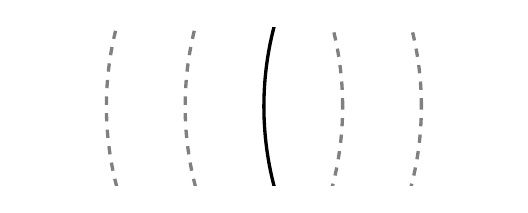
\begin{tikzpicture}
    \clip (1,-1) rectangle (7,1);
    \pgfmathsetmacro{\w}{1}	%scale
	\pgfmathsetmacro{\a}{4}
	\pgfmathsetmacro{\b}{1}

    \coordinate (A) at (0,0);
    \coordinate (A2) at ($(A) + (1,0)$);
    \coordinate (A3) at ($(A2) + (1,0)$);
    \coordinate (B) at (7,0);
    \coordinate (B2) at ($(B) - (1,0)$);
    \coordinate (B3) at ($(B2) - (1,0)$);
    \coordinate (A7) at ($(B3) + (90:\a*\w)$);
    \coordinate (A8) at ($(A7) + (150:\a*\w)$);
    \coordinate (A9) at ($(A8) + (60:\b*\w)$);
    \coordinate (A10) at ($(A9) + (120:\b*\w)$);
    \coordinate (A11) at ($(A10) + (-150:\a*\w)$);
    \coordinate (A12) at ($(A11) + (-90:\a*\w)$);
    \coordinate (A13) at ($(A12) + (180:\b*\w)$);
    \coordinate (A14) at ($(A13) + (-120:\b*\w)$);

	\draw[very thick] (8,0) circle [radius=\a cm];
	\draw[gray,very thick,dashed] (A2) circle [radius=\a cm];
	\draw[gray,very thick,dashed] (A3) circle [radius=\a cm];
	\draw[gray,very thick,dashed] (B) circle [radius=\a cm];
	\draw[gray,very thick,dashed] (B2) circle [radius=\a cm];
\end{tikzpicture}
\end{document}
